\section{Build a Conversational AI System with
  Jaseci}\label{build-a-conversational-ai-system-with-jaseci}

In this tutorial, you are going to learn how to build a state-of-the-art
conversational AI system with Jaseci. You will learn the basics of
Jaseci, training state-of-the-art AI models, and everything between, in
order to create an end-to-end fully-functional conversational AI system.

Excited? Hell yeah! Let's jump in.

\subsection{Preparation}\label{preparation}

To install jaseci, run in your development environment

\begin{verbatim}
pip install jaseci
\end{verbatim}

To test the installation is successful, run

\begin{verbatim}
jsctl -- help
\end{verbatim}

\texttt{jsctl} stands for the Jaseci Command Line Interface. If the
command above displays the help menu for \texttt{jsctl}, then you have
succssfully installed jaseci.

\begin{quote}
    \textbf{Note}

    Take a look and get familiarized with these commands while you are at
    it. \texttt{jsctl} will be frequently used throughout this journey.
\end{quote}

\subsection{Background}\label{background}

A few essential concepts to get familiar with.

\subsubsection{Graph, nodes, edges}\label{graph-nodes-edges}

Link to bible sections.

\subsubsection{Walker}\label{walker}

Link to bible sections.

\section{Automated FAQ answering
  chatbot}\label{automated-faq-answering-chatbot}

Our conversational AI system will consists of multiple components. To
start, we are going to build a chatbot that can answer FAQ questions
without any custom training, using zeroshot NLP models. At the end of
this section, you will have a chatbot that, when given a question,
searches in its knowledge base the most relevant answer and return that
answer.

The use case here is a Tesla FAQ chatbot. We will be using the list of
FAQs from https://www.tesla.com/en\_SG/support/faq.

\begin{quote}
    \textbf{Note}

    This architecture works for any FAQ topics and use case. Feel free to
    pick another product/website/company's FAQ if you'd like!
\end{quote}

\subsection{Define the Nodes}\label{define-the-nodes}

We have 3 different type of nodes:

\begin{itemize}
    \tightlist
    \item
          \texttt{root}: This is the root node of the graph. It is a built-in
          node type and each graph has one root node only.
    \item
          \texttt{faq\_root}: This is the entry point of the FAQ handler. We
          will make the decision on the most relevant answer at this node.
    \item
          \texttt{faq\_state}: This node represents a FAQ entry. It contains a
          candidate answer from the knowledge base.
\end{itemize}

Now let's define the custom node types.

\begin{Shaded}
    \begin{Highlighting}[]
        \NormalTok{node faq_root}\OperatorTok{;}
        \NormalTok{node faq_state }\OperatorTok{\{}
        \NormalTok{    has question}\OperatorTok{;}
        \NormalTok{    has answer}\OperatorTok{;}
        \OperatorTok{\}}
    \end{Highlighting}
\end{Shaded}

The \texttt{has} keyword defines nodes variables. In this case, each
\texttt{faq\_state} has a \texttt{question} and \texttt{answer}.

\begin{quote}
    \textbf{Warning}

    The \texttt{root} node does not need explicit definition. It is a
    built-in node type. Avoid using \texttt{root} as a custom node type.
\end{quote}

To spawn a node of a specific type, use the \texttt{spawn} keyword:

\begin{Shaded}
    \begin{Highlighting}[]
        \NormalTok{faq_answer_1 }\OperatorTok{=}\NormalTok{ spawn node}\OperatorTok{::}\AttributeTok{faq_state}\NormalTok{(}
        \NormalTok{    question}\OperatorTok{=}\StringTok{"How do I configure my order?"}\OperatorTok{,}
        \NormalTok{    answer}\OperatorTok{=}\StringTok{"To configure your order, log into your Tesla account."}\OperatorTok{,}
        \NormalTok{)}\OperatorTok{;}
    \end{Highlighting}
\end{Shaded}

In the above example, we just spawned a \texttt{faq\_state} node called
\texttt{faq\_answer\_1} and initialized its \texttt{question} and
\texttt{answer} variables.

\begin{quote}
    \textbf{Note}

    The \texttt{spawn} keyword can be used to spawn many different jaseci
    objects, such as nodes, graphs and walkers.
\end{quote}

\subsection{Build the Graph}\label{build-the-graph}

For this FAQ chatbot, we will build a graph like illustrated here:

\begin{figure}
    \centering
    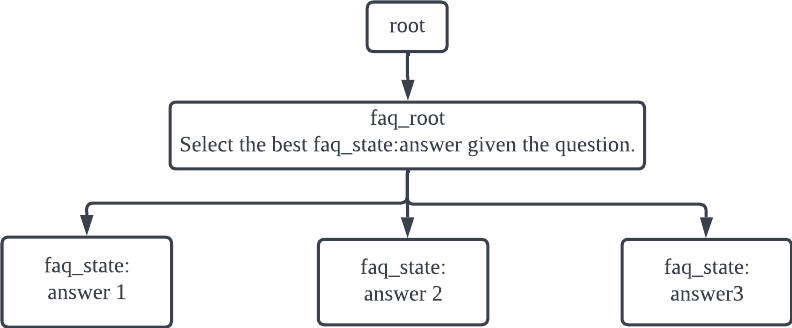
\includegraphics{new_images/faq_1.png}
    \caption{Architecture of FAQ Bot}
\end{figure}

The idea here is that we will decide which FAQ entry is the most
relevant to the incoming question at the \texttt{faq\_root} node and
then we will traverse to that node to fetch the corresponding answer.

To define this graph architecture:

\begin{Shaded}
    \begin{Highlighting}[]
        \CommentTok{// Static graph definition}
        \NormalTok{graph faq }\OperatorTok{\{}
        \NormalTok{    has anchor faq_root}\OperatorTok{;}
        \NormalTok{    spawn }\OperatorTok{\{}
        \CommentTok{// Spawning the nodes}
        \NormalTok{        faq_root }\OperatorTok{=}\NormalTok{ spawn }\DataTypeTok{node}\OperatorTok{::}\NormalTok{faq_root}\OperatorTok{;}
        \NormalTok{        faq_answer_1 }\OperatorTok{=}\NormalTok{ spawn }\DataTypeTok{node}\OperatorTok{::}\AttributeTok{faq_state}\NormalTok{(}
        \NormalTok{            question}\OperatorTok{=}\StringTok{"How do I configure my order?"}\OperatorTok{,}
        \NormalTok{            answer}\OperatorTok{=}\StringTok{"To configure your order, log into your Tesla account."}
        \NormalTok{        )}\OperatorTok{;}
        \NormalTok{        faq_answer_2 }\OperatorTok{=}\NormalTok{ spawn }\DataTypeTok{node}\OperatorTok{::}\AttributeTok{faq_state}\NormalTok{(}
        \NormalTok{            question}\OperatorTok{=}\StringTok{"How do I order a tesla"}\OperatorTok{,}
        \NormalTok{            answer}\OperatorTok{=}\StringTok{"Visit our design studio to place your order."}
        \NormalTok{        )}\OperatorTok{;}
        \NormalTok{        faq_answer_3 }\OperatorTok{=}\NormalTok{ spawn }\DataTypeTok{node}\OperatorTok{::}\AttributeTok{faq_state}\NormalTok{(}
        \NormalTok{            question}\OperatorTok{=}\StringTok{"Can I request a test drive"}\OperatorTok{,}
        \NormalTok{            answer}\OperatorTok{=}\StringTok{"Yes. You must be a minimum of 25 years of age."}
        \NormalTok{        )}\OperatorTok{;}

        \CommentTok{// Connecting the nodes together}
        \NormalTok{        faq_root }\OperatorTok{-->}\NormalTok{ faq_answer_1}\OperatorTok{;}
        \NormalTok{        faq_root }\OperatorTok{-->}\NormalTok{ faq_answer_2}\OperatorTok{;}
        \NormalTok{        faq_root }\OperatorTok{-->}\NormalTok{ faq_answer_3}\OperatorTok{;}
        \OperatorTok{\}}
        \OperatorTok{\}}
    \end{Highlighting}
\end{Shaded}

Let's break down this piece of code.

\begin{itemize}
    \tightlist
    \item
          We spawn 4 nodes, one of the type \texttt{faq\_root} and three are of
          the type \texttt{faq\_state}.
    \item
          We connect each of the faq answer state to the faq root with
          \texttt{faq\_root\ -\/-\textgreater{}\ faq\_answer\_*}.
    \item
          We set the \texttt{faq\_root} as the anchor node of the graph.
          Spawning a graph will return its anchor node.
\end{itemize}

\begin{quote}
    \textbf{Warning}

    An anchor node is required for a graph block. It must be spawned inside
    the spawn block of the graph definition.
\end{quote}

\subsection{Initialize the Graph}\label{initialize-the-graph}

Similar to nodes, in order to create the graph, we will use the
\texttt{spawn} keyword.

\begin{Shaded}
    \begin{Highlighting}[]
        \NormalTok{walker init }\OperatorTok{\{}
        \NormalTok{    root }\OperatorTok{\{}
        \NormalTok{        spawn here }\OperatorTok{-->} \DataTypeTok{graph}\OperatorTok{::}\NormalTok{faq}\OperatorTok{;}
        \OperatorTok{\}}
        \OperatorTok{\}}
    \end{Highlighting}
\end{Shaded}

This is the first walker we have introduced so let's break it down.

\begin{itemize}
    \tightlist
    \item
          The walker is called \texttt{init}.
    \item
          It contains logic specifically for the \texttt{root} node, meaning
          that the code inside the \texttt{root\ \{\}} block will run
          \textbf{only} on the \texttt{root} node. This syntax applies for any
          node types, as you will see very soon.
    \item
          \texttt{spawn\ here\ -\/-\textgreater{}\ graph::faq} creates an
          instance of the \texttt{faq} graph and connect its anchor node to
          \texttt{here} which is the node the walker is currently on.
\end{itemize}

\begin{quote}
    \textbf{Note}

    \texttt{init} is a built-in walker type. It is the default walker to run
    when no specific walkers are specified for a \texttt{jac\ run} command.

    \texttt{here} is a very powerful keyword. It always evaluates to the
    specific node the walker is currently on. You will be using
    \texttt{here} a lot throughout this tutorial.
\end{quote}

\subsection{\texorpdfstring{Run the \texttt{init}
        Walker}{Run the init Walker}}\label{run-the-init-walker}

Now, let's run the init walker to initialize the graph. First put all
the above code snippet in a single jac file and name it
\texttt{main.jac}, including

\begin{itemize}
    \tightlist
    \item
          nodes defintion
    \item
          graph definition
    \item
          init walker
\end{itemize}

Run \texttt{jsctl} to get into the jaseci shell environment:

\begin{Shaded}
    \begin{Highlighting}[]
        \ExtensionTok{jsctl}
    \end{Highlighting}
\end{Shaded}

Inside the \texttt{jsctl} shell,

\begin{Shaded}
    \begin{Highlighting}[]
        \ExtensionTok{jaseci} \OperatorTok{>}\NormalTok{ jac dot main.jac}
    \end{Highlighting}
\end{Shaded}

This command runs the \texttt{init} walker of the \texttt{main.jac}
program and return the state of its graph in DOT format after the walker
has finished. \href{https://graphviz.org/doc/info/lang.html}{The DOT
    language} is a popular graph description language widely used for
representing complex graphs.

The output should look something like this

\begin{Shaded}
    \begin{Highlighting}[]
        \VariableTok{strict} \KeywordTok{digraph} \VariableTok{root} \OtherTok{\{}
        \CommentTok{    }\StringTok{"n0"}\CommentTok{ }\OtherTok{[}\CommentTok{ }\VariableTok{id}\OtherTok{=}\StringTok{"0955c04e4ff945b4b836748ef2bbd98a"}\CommentTok{, }\AttributeTok{label}\OtherTok{=}\StringTok{"n0:root"}\CommentTok{  }\OtherTok{]}
        \CommentTok{    }\StringTok{"n1"}\CommentTok{ }\OtherTok{[}\CommentTok{ }\VariableTok{id}\OtherTok{=}\StringTok{"c1240d79110941c1bc2feb18581951bd"}\CommentTok{, }\AttributeTok{label}\OtherTok{=}\StringTok{"n1:faq_state"}\CommentTok{  }\OtherTok{]}
        \CommentTok{    }\StringTok{"n2"}\CommentTok{ }\OtherTok{[}\CommentTok{ }\VariableTok{id}\OtherTok{=}\StringTok{"55333be285c246db88181ac34d16cd20"}\CommentTok{, }\AttributeTok{label}\OtherTok{=}\StringTok{"n2:faq_state"}\CommentTok{  }\OtherTok{]}
        \CommentTok{    }\StringTok{"n3"}\CommentTok{ }\OtherTok{[}\CommentTok{ }\VariableTok{id}\OtherTok{=}\StringTok{"d4fa8f2c46ca463f9237ef818e086a29"}\CommentTok{, }\AttributeTok{label}\OtherTok{=}\StringTok{"n3:faq_state"}\CommentTok{  }\OtherTok{]}
        \CommentTok{    }\StringTok{"n4"}\CommentTok{ }\OtherTok{[}\CommentTok{ }\VariableTok{id}\OtherTok{=}\StringTok{"f7b1c8ae82af4063ad53646adc5544e9"}\CommentTok{, }\AttributeTok{label}\OtherTok{=}\StringTok{"n4:faq_state"}\CommentTok{  }\OtherTok{]}
        \CommentTok{    }\StringTok{"n0"}\CommentTok{ }\OtherTok{->}\CommentTok{ }\StringTok{"n1"}\CommentTok{ }\OtherTok{[}\CommentTok{ }\VariableTok{id}\OtherTok{=}\StringTok{"a718fd6c938149269d3ade2af2eb023c"}\CommentTok{, }\AttributeTok{label}\OtherTok{=}\StringTok{"e0"}\CommentTok{ }\OtherTok{]}
        \CommentTok{    }\StringTok{"n1"}\CommentTok{ }\OtherTok{->}\CommentTok{ }\StringTok{"n2"}\CommentTok{ }\OtherTok{[}\CommentTok{ }\VariableTok{id}\OtherTok{=}\StringTok{"3757cb15851249b4b6083d7cb3c34f8e"}\CommentTok{, }\AttributeTok{label}\OtherTok{=}\StringTok{"e1"}\CommentTok{ }\OtherTok{]}
        \CommentTok{    }\StringTok{"n1"}\CommentTok{ }\OtherTok{->}\CommentTok{ }\StringTok{"n4"}\CommentTok{ }\OtherTok{[}\CommentTok{ }\VariableTok{id}\OtherTok{=}\StringTok{"626ce784a8f5423cae5d5d5ca857fc5c"}\CommentTok{, }\AttributeTok{label}\OtherTok{=}\StringTok{"e2"}\CommentTok{ }\OtherTok{]}
        \CommentTok{    }\StringTok{"n1"}\CommentTok{ }\OtherTok{->}\CommentTok{ }\StringTok{"n3"}\CommentTok{ }\OtherTok{[}\CommentTok{ }\VariableTok{id}\OtherTok{=}\StringTok{"a609e7b54bde4a6a9c9711afdb123241"}\CommentTok{, }\AttributeTok{label}\OtherTok{=}\StringTok{"e3"}\CommentTok{ }\OtherTok{]}
        \OtherTok{\}}
    \end{Highlighting}
\end{Shaded}

\begin{quote}
    \textbf{Note}

    We are not going to cover the DOT syntax. There are many resources
    online if you are interested, e.g.,
    https://graphviz.org/doc/info/lang.html
\end{quote}

\begin{quote}
    \textbf{Note}

    There are tools available to render a graph in DOT format. For example,
    https://dreampuf.github.io/GraphvizOnline has as WSIWYG editor to render
    dot graph in real time.
\end{quote}

Congratulations! 🎉 You have just created your first functional jac
program!

\subsection{Ask the Question}\label{ask-the-question}

Alright, we have initialized the graph. Now it's time to create the code
for the question-answering. We will start with a simple string matching
for the answer selection algorithm. For this, we will create a new
walker called \texttt{ask}.

\begin{Shaded}
    \begin{Highlighting}[]
        \NormalTok{walker ask }\OperatorTok{\{}
        \NormalTok{    has question}\OperatorTok{;}
        \NormalTok{    root }\OperatorTok{\{}
        \NormalTok{        question }\OperatorTok{=} \VariableTok{std}\NormalTok{.}\AttributeTok{input}\NormalTok{(}\StringTok{">"}\NormalTok{)}\OperatorTok{;}
        \NormalTok{        take }\OperatorTok{-->} \DataTypeTok{node}\OperatorTok{::}\NormalTok{faq_root}\OperatorTok{;}
        \OperatorTok{\}}
        \NormalTok{    faq_root }\OperatorTok{\{}
        \NormalTok{        take }\OperatorTok{-->} \DataTypeTok{node}\OperatorTok{::}\AttributeTok{faq_state}\NormalTok{(question}\OperatorTok{=}\NormalTok{question)}\OperatorTok{;}
        \OperatorTok{\}}
        \NormalTok{    faq_state }\OperatorTok{\{}
        \VariableTok{std}\NormalTok{.}\AttributeTok{out}\NormalTok{(}\VariableTok{here}\NormalTok{.}\AttributeTok{answer}\NormalTok{)}\OperatorTok{;}
        \OperatorTok{\}}
        \OperatorTok{\}}
    \end{Highlighting}
\end{Shaded}

This walker is more complex than the \texttt{init} one and introduces a
few new concepts so let's break it down!

\begin{itemize}
    \tightlist
    \item
          Similar to nodes, walker can also contain \texttt{has} variables. They
          define variables of the walker. They can also be passed as parameters
          when calling the walker.
    \item
          \texttt{std.input} and \texttt{std.out} read and write to the command
          line.
    \item
          This walker has logic for three types of node: \texttt{root},
          \texttt{faq\_root} and \texttt{faq\_state}.
    \item
          \texttt{root}: It simply traverse to the \texttt{faq\_root} node.
    \item
          \texttt{faq\_root}: This is where the answer selection algorim is. We
          will find the most relevant \texttt{faq\_state} and then traverse to
          that node via a \texttt{take} statement. In this code snippet, we are
          using a very simple (and limited) string matching approach to try to
          match the predefined FAQ question with the user question.
    \item
          \texttt{faq\_state}: Print the answer to the terminal
\end{itemize}

Before we run this walker, we are going to update the \texttt{init}
walker to speed up our development process

\begin{Shaded}
    \begin{Highlighting}[]
        \NormalTok{walker init }\OperatorTok{\{}
        \NormalTok{    root }\OperatorTok{\{}
        \NormalTok{        spawn here }\OperatorTok{-->} \DataTypeTok{graph}\OperatorTok{::}\NormalTok{faq}\OperatorTok{;}
        \NormalTok{        spawn here }\DataTypeTok{walker}\OperatorTok{::}\NormalTok{ask}\OperatorTok{;}
        \OperatorTok{\}}
        \OperatorTok{\}}
    \end{Highlighting}
\end{Shaded}

This serves as a shorthand so that we can initialize the graph and ask
question in one command.

\begin{quote}
    \textbf{Note}

    This demonstrates how one walker can spawn another walker using the
    \texttt{spawn} keyword.
\end{quote}

Time to run the walker!

\begin{Shaded}
    \begin{Highlighting}[]
        \ExtensionTok{jaseci} \OperatorTok{>}\NormalTok{ jac run main.jac}
    \end{Highlighting}
\end{Shaded}

\texttt{jac\ run} functions very similarly to \texttt{jac\ dot}, with
the only difference being that it doesn't return the graph in DOT
format. Try giving it one of the three questions we have predefined and
it should respond with the corresponding answer.

\subsection{Introducing Universal Sentence
    Encoder}\label{introducing-universal-sentence-encoder}

Now, obvisouly, what we have now is not very ``AI'' and we need to fix
that. We are using the Universal Sentence Encoder QA model as the answer
selection algorithm. Universal Sentence Encoder is a language encoder
model that is pre-trained on large corpus of natural language data and
have been shown to be effective in many NLP tasks. In our application,
we are using it for zero-shot question-answering, i.e.~no custom
training required.

Jaseci has a set of built-in libraries or packages that are called
Jaseci actions. These actions cover a wide-range of state-of-the-art AI
models across many different NLP tasks. These actions are packaged in a
python module called \texttt{jaseci\_kit}.

To install \texttt{jaseci\_kit}:

\begin{Shaded}
    \begin{Highlighting}[]
        \ExtensionTok{pip}\NormalTok{ install jaseci_kit}
    \end{Highlighting}
\end{Shaded}

Now we load the action we need into our jaseci environment

\begin{Shaded}
    \begin{Highlighting}[]
        \ExtensionTok{jaseci} \OperatorTok{>}\NormalTok{ actions load module jaseci_kit.use_qa}
    \end{Highlighting}
\end{Shaded}

Let's update our walker logic to use the USE QA model:

\begin{Shaded}
    \begin{Highlighting}[]
        \NormalTok{walker ask }\OperatorTok{\{}
        \NormalTok{    has question}\OperatorTok{;}
        \NormalTok{    root }\OperatorTok{\{}
        \NormalTok{        question }\OperatorTok{=} \VariableTok{std}\NormalTok{.}\AttributeTok{input}\NormalTok{(}\StringTok{">"}\NormalTok{)}\OperatorTok{;}
        \NormalTok{        take }\OperatorTok{-->} \DataTypeTok{node}\OperatorTok{::}\NormalTok{faq_state}\OperatorTok{;}
        \OperatorTok{\}}
        \NormalTok{    faq_root }\OperatorTok{\{}
        \NormalTok{        answers }\OperatorTok{=} \OperatorTok{-->}\NormalTok{.}\AttributeTok{answer}\OperatorTok{;}
        \NormalTok{        best_answer }\OperatorTok{=} \VariableTok{use}\NormalTok{.}\AttributeTok{qa_classify}\NormalTok{(}
        \NormalTok{            text }\OperatorTok{=}\NormalTok{ question}\OperatorTok{,}
        \NormalTok{            classes }\OperatorTok{=}\NormalTok{ answers}
        \NormalTok{        )}\OperatorTok{;}
        \NormalTok{        take }\OperatorTok{-->} \DataTypeTok{node}\OperatorTok{::}\AttributeTok{faq_state}\NormalTok{(answer}\OperatorTok{==}\NormalTok{best_answer[}\StringTok{"matched"}\NormalTok{])}\OperatorTok{;}
        \OperatorTok{\}}
        \NormalTok{    faq_state }\OperatorTok{\{}
        \VariableTok{std}\NormalTok{.}\AttributeTok{out}\NormalTok{(}\VariableTok{here}\NormalTok{.}\AttributeTok{answer}\NormalTok{)}\OperatorTok{;}
        \OperatorTok{\}}
        \OperatorTok{\}}
    \end{Highlighting}
\end{Shaded}

Even though there are only 5 lines of new code, there are many
interesting aspects so let's break it down!

\begin{itemize}
    \tightlist
    \item
          \texttt{-\/-\textgreater{}.answer} collects the \texttt{answer}
          variable of all of the nodes that are connected to
          \texttt{here}/\texttt{faq\_root} with a \texttt{-\/-\textgreater{}}
          connection.
    \item
          \texttt{use.qa\_classify} is one of the action supported by the USE QA
          action set. It takes in a question and a list of candidate answers and
          return the most relevant one.
\end{itemize}

Now let's run this new walker and you can now ask questions that are
relevant to the answers beyond just the predefined ones.

\subsection{Scale it Out}\label{scale-it-out}

So far we have created a FAQ bot that is capble of provide answer in
three topics. To make this useful beyond just a prototype, we are now
going to expand its database of answers. Instead of manually spawning
and connecting a node for each FAQ entry, we are going to write a walker
that automatically expand our graph:

\begin{Shaded}
    \begin{Highlighting}[]
        \NormalTok{walker ingest_faq }\OperatorTok{\{}
        \NormalTok{    has kb_file}\OperatorTok{;}
        \DataTypeTok{root}\OperatorTok{:}\NormalTok{ take }\OperatorTok{-->} \DataTypeTok{node}\OperatorTok{::}\NormalTok{faq_root}\OperatorTok{;}
        \NormalTok{    faq_root }\OperatorTok{\{}
        \NormalTok{        kb }\OperatorTok{=} \VariableTok{file}\NormalTok{.}\AttributeTok{load_json}\NormalTok{(kb_file)}\OperatorTok{;}
        \ControlFlowTok{for}\NormalTok{ faq }\KeywordTok{in}\NormalTok{ kb }\OperatorTok{\{}
        \NormalTok{            answer }\OperatorTok{=}\NormalTok{ faq[}\StringTok{"answer"}\NormalTok{]}\OperatorTok{;}
        \NormalTok{            spawn here }\OperatorTok{-->} \DataTypeTok{node}\OperatorTok{::}\AttributeTok{faq_state}\NormalTok{(answer}\OperatorTok{=}\NormalTok{answer)}\OperatorTok{;}
        \OperatorTok{\}}
        \OperatorTok{\}}
        \OperatorTok{\}}
    \end{Highlighting}
\end{Shaded}

\begin{quote}
    \textbf{Note}

    If are curious (and adventurous), try visualizes this new graph via DOT!
\end{quote}
